\paragraph{Sơ đồ tuần tự luồng thu hồi chia sẻ cuộc trò chuyện}

Luồng nghiệp vụ này mô tả
vòng đời của một yêu cầu thu hồi quyền chia sẻ cuộc trò chuyện từ người dùng,
đảm bảo tính nhất quán dữ liệu giữa
các dịch vụ thông qua mẫu thiết kế Transactional Outbox và giao tiếp bất đồng bộ qua RabbitMQ.

\begin{figure}[H]
\centering
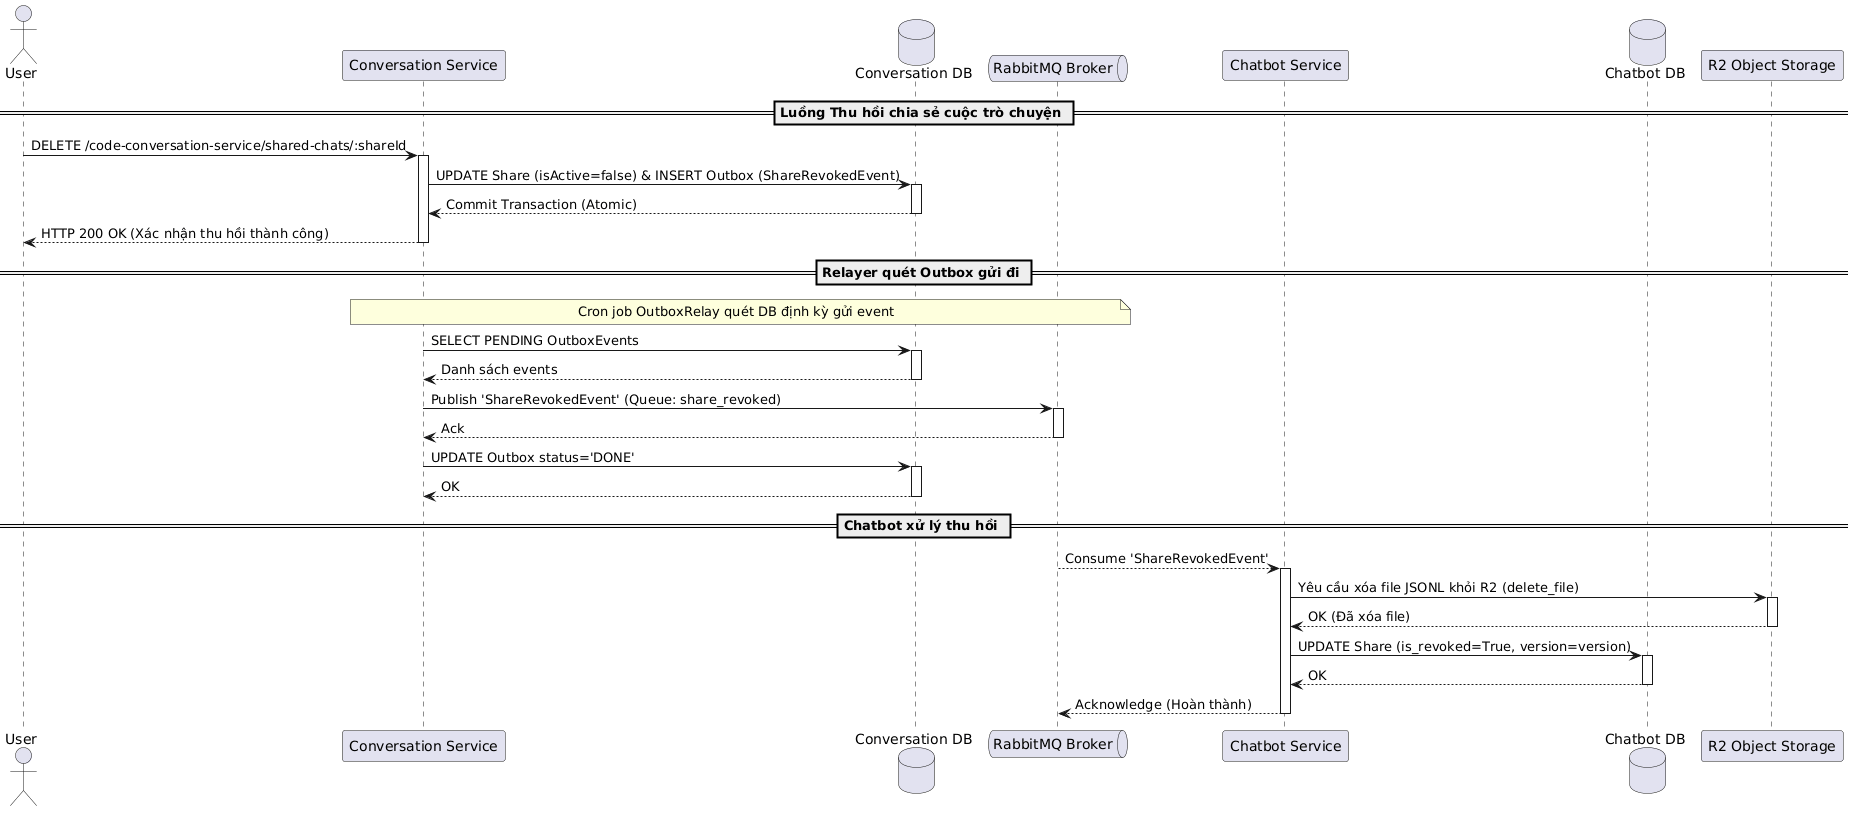
\includegraphics[width=0.95\textwidth]{contents/Sequence/UML-Sequence-UserRevokeSharedChat.png}
\caption{Sơ đồ tuần tự luồng thu hồi chia sẻ cuộc trò chuyện}
\end{figure}

\subparagraph{Mô tả tổng quan}

\begin{itemize}

\item \textbf{Yêu cầu hủy chia sẻ:}
Người dùng gửi yêu cầu hủy quyền chia sẻ
cuộc trò chuyện thông qua giao diện.

\item \textbf{Cập nhật bản ghi chia sẻ:}
Dịch vụ trò chuyện
thực hiện cập nhật trạng thái liên kết chia sẻ thành ngừng hoạt động,
đồng thời ghi nhận sự kiện hủy chia sẻ vào
bảng sự kiện chờ gửi trong cùng một giao dịch CSDL để đảm bảo tính nhất quán.

\item \textbf{Phản hồi kết quả:}
Dịch vụ phản hồi kết quả hủy chia sẻ thành công
về giao diện người dùng ngay lập tức để giảm thời gian chờ.

\item \textbf{Gửi thông điệp hủy:}
Tiến trình chuyển tin nhắn
quét bảng sự kiện chờ gửi định kỳ,
lấy sự kiện hủy chia sẻ và gửi thông điệp vào hàng đợi tin nhắn.

\item \textbf{Xóa tệp tin chia sẻ:}
Dịch vụ chatbot nhận thông điệp hủy chia sẻ từ hàng đợi tin nhắn,
tiến hành xóa tệp tin lưu trữ cuộc trò chuyện tương ứng trên kho lưu trữ trực tuyến ngay lập tức.

\item \textbf{Hoàn tất cập nhật:}
Dịch vụ chatbot cập nhật trạng thái liên kết chia sẻ
trong CSDL chatbot thành đã hủy và gửi xác nhận hoàn thành xử lý.
\end{itemize}

\begin{table}[H]
\centering
\renewcommand{\arraystretch}{1.3}

\begin{tabular}{|l|l|p{5cm}|}
\hline
\textbf{Thành phần} & \textbf{Phân loại} & \textbf{Vai trò trong hệ thống} \\ \hline
User & Actor & Người dùng khởi tạo yêu cầu thu hồi quyền chia sẻ cuộc trò chuyện. \\ \hline
Conversation Service & Microservice & Dịch vụ tiếp nhận yêu cầu từ người dùng, thực hiện cập nhật CSDL và ghi lại sự kiện vào bảng Outbox. \\ \hline
Conversation DB & Database & CSDL chính của Conversation Service, lưu trữ trạng thái bản ghi chia sẻ (Share) và bảng hàng đợi sự kiện (Outbox). \\ \hline
RabbitMQ Broker & Message Broker & Message Broker nhận sự kiện và phân phối đến các dịch vụ theo dõi. \\ \hline
Chatbot Service & Microservice & Dịch vụ đóng vai trò là Consumer, lắng nghe sự kiện từ RabbitMQ, thực thi nghiệp vụ xóa file và cập nhật CSDL. \\ \hline
Chatbot DB & Database & CSDL của Chatbot Service, dùng để lưu trữ trạng thái bản ghi chia sẻ và cơ chế kiểm soát phiên bản. \\ \hline
R2 Object Storage & External Service & Dịch vụ lưu trữ đối tượng lưu trữ vật lý các tệp tin dữ liệu cuộc trò chuyện định dạng JSONL. \\ \hline
\end{tabular}
\caption{Các thành phần tham gia luồng thu hồi chia sẻ cuộc trò chuyện}
\end{table}
